% Niveau :      PC
% Discipline :  Méca
% Mots clés :   Pont suspendu

\begin{exercise}{Pont suspendu}{2}{Sup, Spé}
{Mécanique, Ondes mécaniques, Corde}{bermu}

Soit un pont suspendu enjambant un bras de mer, maintenu par un câble de poids négligeable attaché à deux poteaux de hauteur $H$ plantés de part et d'autre du pont et séparés d'une longeur $L$.

\begin{figure}[H]
    \centering
    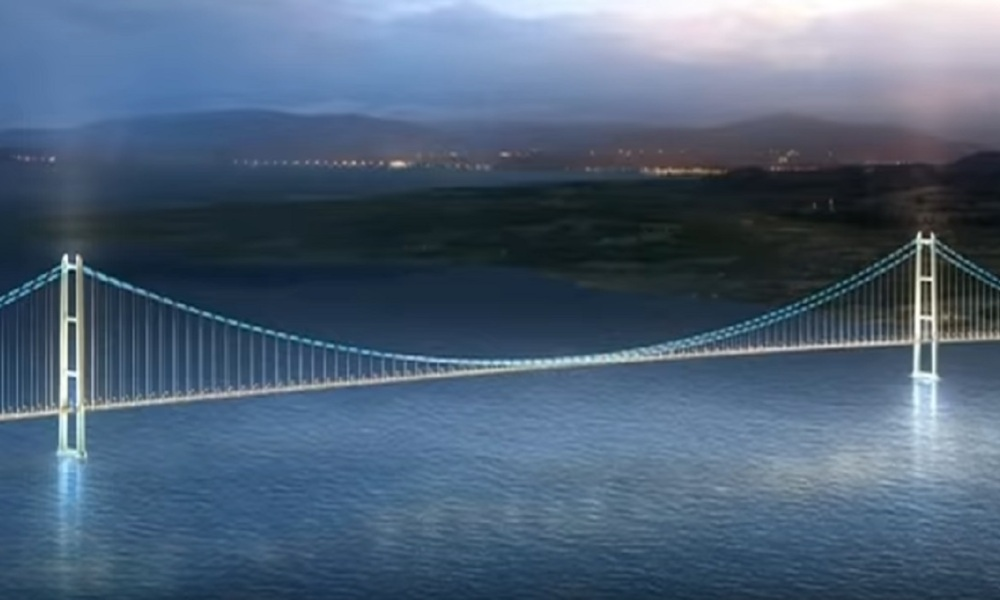
\includegraphics[height=15em]{meca/ondes_meca/pont-suspendu.jpeg}
    \caption{Vision d'artiste du projet du plus grand pont suspendu du monde, en Turquie.}
\end{figure}

\begin{questions}
\question Donner l'équation décrivant la forme du câble.
\uplevel{On s'intéresse maintenant au tablier du pont (la partie où se trouve la route) qui, lorsque le pont est au repos, est horizontal.}
\question Montrez que la hauteur du tablier vérifie une équation d'onde. On précisera la célérité associée.
\question Dans quel cas le tablier peut-il entrer en résonance ? Citer un cas célèbre où un tel phénomène s'est produit.
\end{questions}

\paragraph{Données :}  L’abscisse curviligne $s$ est telle qu’un élément de longueur de la corde $\dd{s}$ de la courbe vérifie
\begin{align*}
    \dd{s}^2 = \dd{x}^2 + \dd{z}^2 &= \qty(1+ z'(x)^2)\dd{x}^2.
\end{align*}
\end{exercise}